\section{Collision Avoidance} \label{sec:collision_avoidance}

\subsection{Inertia Drift}
Let us assume that have strong damping in the direction of the obstacle, i.e., $s^{\mathrm{obs}} / m_i \gg 1$, where $m_i$ with $i = 1, .., N$ represent the eigenvalues of the mass matrix $\matd{M}$. 


\subsection{Disturbance Repulsion}
Let us assume a disturbance impact at time $t_0$, which results in the robot having an impact velocity of $\vecs{\dot \xi} = \vect v^I$, which is pointing towards the obstacle. The impact velocity is much larger than the robot's initial velocity. Thus the latter is neglected, and the obstacle is approximated as locally flat and the velocity locally constant (see Fig.~\ref{fig:collision_avoidance}). Furthermore, we assume to be close to the robot, i.e., $\Gamma(\vecs \xi) \approx 1$, hence the $w(\vecs \xi) \approx 1$, and the stiffness in the direction of the obstacle is approximated as $s^{\mathrm{obs}}$.
No further impact forces are applied after the initial impact is absorbed. The Coriolis effect is neglected in the short time frame.

\begin{lemma}
	Using the control law in continuous time, ...
\end{lemma}

\begin{proof}
The velocity with the controller can be analyzed as follows:
\begin{equation}
    \vecs{\dot \xi} = \int \vecs{\ddot \xi} \, dt = \int \matd{M}^{-1} \matd{D}  \left( \vecs{\dot \xi} - \vecs f(\vecs \xi) \right) \, dt
\end{equation}

Let us analyze when the decoupled velocity along the normal reaches zero:
\begin{equation}
    \vecs{\dot \xi} = \int \frac{s^{\mathrm{obs}}}{m} \vecs{\dot \xi} \, dt = \frac{s^{\mathrm{obs}}}{m} \vecs{\xi} + \vecs v^I \label{eq:velocity_with_control}
\end{equation}
The velocity along the normal reaches zero at position, i.e., 
\begin{equation}
    \| \vecs{\dot \xi} \| = 0
    \quad \Rightarrow \quad
    \|\vecs{\xi} \| = \| \vecs v^I \| {m} / {s^{\mathrm{obs}}} 
\end{equation}

The statement follows directly from \eqref{eq:velocity_with_control}.
\end{proof}

\subsection{Disturbance Repulsion with Force Limit}
Robotic systems have a maximum force that can be exerted based on the motors and their geometry, $\tau_c^{\mathrm{max}} \in \mathbb{R}_{>0}$. Note that this maximum might be state dependent.

Let  us assume strong damping concerning the maximum force, i.e., $s^{\mathrm{obs}} / \tau_c^{\mathrm{max}} \gg 1$, hence we can assume that the magnitude of the obstacle repulsive force is equal to the maximum force close to the obstacle. Hence, the maximum disturbance.

\subsection{Practical Considerations}
As described in \cite{huber2022avoiding, huber2023avoidance}, the avoidance velocity when approaching an obstacle can be directed along the normal of the obstacle to point away from the surface when reaching the obstacle and inside. This allows improved recovery, for scenarios such as those presented.

\begin{figure}
\centering
\begin{subfigure}{0.99\columnwidth}
  \centerline{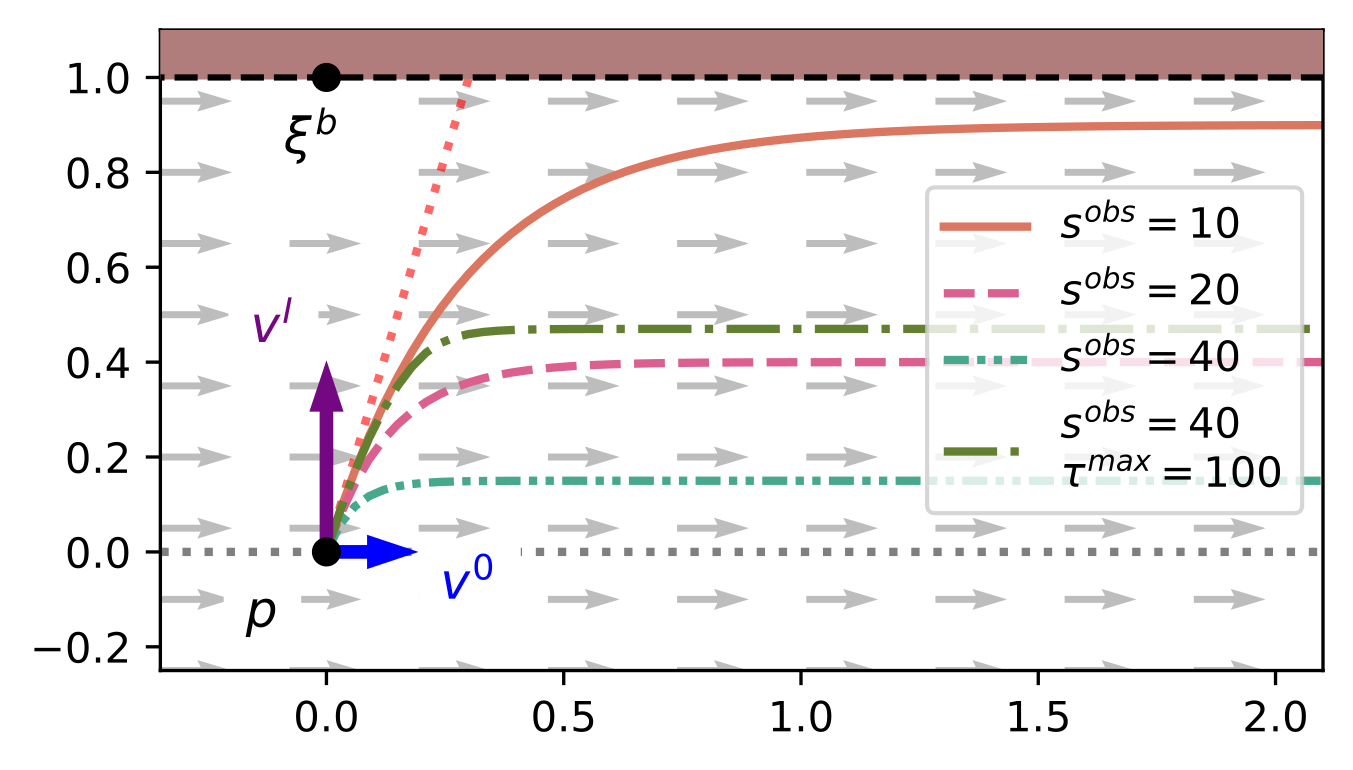
\includegraphics[width=\textwidth]{figures/parallel_avoidance_obstacle}}
  \caption{Parallel to surface velocity}
  \label{fig:disturbance_with_parallel_velocity}
\end{subfigure}
\begin{subfigure}{0.5\columnwidth}
  %% \centerline{\includegraphics[width=\textwidth]{}}
  \caption{Repulsive surface velocity}
  \label{fig:disturbance_with_repulsive_velocity}
\end{subfigure}
\caption{Comparison of the two control methods}
\label{fig:disturbance_rejection_schematics}
\end{figure}


